% !TeX root = ../my-thesis.tex
\chapter{Einleitung}

\section{Motivation}
Die Motivation für die Erarbeitung der Forschungsfrage ergab sich am 29. Juni 2020, als eine Rundmail von dem Data Breach Monitoring-Tool von Firefox die Bildschirme erreichte, welches einen neuen Incident bei Wattpad meldete. Wattpad ist eine Webseite, bei welcher Nutzer Geschichten frei für die Öffentlichkeit schreiben und publizieren können. Nun stellt sich die berechtige Frage, inwiefern diese in Relation kleine Webseite verwertbare Daten für einen Angreifer oder ein bösartiges Tool liefern kann. Dazu genügt es sich die Daten genauer anzusehen. Kompromittiert wurden neben den klassichen Daten wie Passwörtern, IP-Adressen, E-Mail-Adressen und Geburtsdaten auch sehr persönliche Informationen wie geografische Standorte, ein Kurzprofil des Nutzers, das Profilbild, die Social-Media-Profile und sogenannte Session-Tokens jeglicher Dienste des Benutzers, die mit Wattpad verknüpft waren. Entnehmen kann man dies mehreren Artikeln, bei der allerdings die Größe der Datenmengen zwischen 250 und 280 Millionen Einträgen variieren. Eine genaue Zahl liefert der Artikel der riskbasedsecurity mit 268.830.266 (nach der Entfernung von Duplikaten) kompromittierten E-Mail Addressen, die sich laut des Artikels in einer einzigen Datenbank befanden. [7] Diese Zahl ist dennoch nur als Richtwert zu verstehen, da wie bereits erwähnt das Ausmaß des Datenlecks bei Wattpad nicht in Gänze bekannt ist.

\section{Problemdefinition}
Die Identität dieser Nutzer hängt an ihrem Passwort, demnach ist die plötzliche Bedrohung für jeden Einzelnen nun allgegenwärtig. Das Passwort, welches nun im Netz ist, ist schwierig bis unmöglich aus allen (Sub-)Quellen eliminierbar. Die Identität der Personen kann nun von Angreifern genutzt werden, um z.B. finanziellen Schaden anzurichten und sich selbst zu bereichern.
\newpage

Auch wenn es teilweise nicht so scheint, ist das Problem mit Passwörtern so alt wie das Internet selbst und Wattpad ist nicht das einzige Beispiel von veröffentlichten Datenlecks der letzten Jahre. Angriffsszenarien auf technischer Seite (Code-Injektionen, 0-Day-Exploits, Bruteforce-Angriffe) scheint die informationsafine Menscheit der Neuzeit gut organisiert zu bekommen, doch dann scheitert es in riesigen Unternehmen oft an der Wahl eines Passwortes einer wichtigen Einzelperson, welches dann in Kettenreaktionen zu solchen Data Breaches und größeren Attacken auf Unternehmen führen.

Bei Disskusionen im Internet, wird sich häufig aufgrund der selben (wiederholenden) Gründe gegen eine zwei Faktor Authentifizierung (2FA) und zusätzliche Sicherheiten für die Passwortwahl ausgesprochen. Die 2FA sei zu umständlich und ein Passwort-Manager aufgrund des Masterpasswortes und der Angst vor einem Massenverlust an Daten zu riskant. Das potenzielle Risiko welches durch Passwörter allerdings im Vergleich zu diesen neueren Verfahren aufkommt, wird häufig ignoriert. Individuelle Passwörter für jeden Dienst seien unmöglich merkbar und eine zwei Faktor Authentifizierung sei nicht bedienfreundlich genug um sie für jeden Dienst einzusetzen. Damit meinen Nutzer die verhältnismäßig lange Zeit, die bis zur erfolgreichen Authentifikation vergeht. Je nach Dienst gibt es nämlich keine Sessionverwaltung, sodass jede Authentifizierung auch einen zweiten Faktor (ein externes Gerät) benötigt, welches natürlich die Dauer des Loginvorgangs beeinträchtigt. Die Frage, die sich stellt ist es, ob man mit einer Kombination aus den vorhandenen vielfältigen Authentifizierungsmöglichkeiten eine beqeueme aber gleichzeitig sichere Authentifizierungsvariante schaffen kann, bei denen es dem Anwender möglich sein soll, sich gegenüber einer Webseite zu authentifizieren.

\section{Stand der Forschung}
\subsection{Unsichere Passwörter}
In der fünften Ausgabe der Zeitschrift ``Wirtschaftsinformatik \& Management''  2018 mit dem Titel ``Schwache Passwörter - Nutzer spielen weiterhin Vogel Strauß'' schrieb der Autor Geralt Beuchelt: ``Der Umgang mit Passwörtern ist so ähnlich wie eine Diät: Eigentlich weiß man genau, was richtig ist - Macht aber oft genug das Gegenteil. Und nicht selten ist der Grund Bequemlichkeit. Warum selber kochen, wann nach einem langen Tag eine Pizza lockt? Und warum lange, umständliche Passwörter verwenden, wenn es einfach zu merkende, die man für alle Accounts verwendet, doch auch tun?'' [3]. Damit greift der Autor sehr zutreffend die Hauptproblematik des Passwortes in der Neuzeit auf.

\newpage

Die symbolische Pizza steht für die Mehrfachverwendung von teils schwachen Passwörtern für alle genutzten Dienste inklusive des 'Verwaltungsdienstes' wie der Mail, welches als meist einziges Identifikationsmerkmal dient, über die weitere Dienste betroffen sein können. Der Begriff des Passwortes stammt aus dem militärischen Bereich des 16. Jahrhunderts, wobei tatsächlich das einzelne Wort addressiert war, welches einem Zutritt zu Gebäuden verschaffte. Damit verwandt ist das Kennwort, welches nicht das Passieren sondern die Kennung des gemeinsamen Geheimnisses betont. Dies bedeutet, dass der Passierer mit einem Kennwort auch automatisch ein Geheimnisträger ist. Als allerdings Computer immer leistungsfähiger wurden, wurde der Begriff der Passphrase etabliert, um die Notwendigkeit längerer Passwörter hervorzuheben. Dies geschah vorallem weil zu dieser Zeit keine Forschung rund um Passwörter betrieben wurde und die Komplexität noch keine Rolle fand. Weitere Schlüsselwörter für das heutzutage bekannte Passwort sind: Schlüsselwort, Kodewort (u.a: Codewort) oder die Parole, diese werden im Folgenden als Synonym für die heutige Passphrase verwendet. Die Länge gillt gemeinhin als die allumfassende Sicherheit von Passwörtern. Dem widerspricht die klare Trennung zwischen Länge und Komplexität von Passwörtern durch das Bundesamt für Sicherheit in der Informationstechnik, die sinngemäß in ihrer Empfehlung zum Thema ``sichere Passwörter`` schreiben, dass die Länge von Passwörtern nicht dessen Komplexität und Sicherheit gegen Angriffe widerspiegelt [4].

Um sichere Passwörter zu erzwingen, setzen Webseiten immer häufiger auf Passwort Policys. Diese machen anhand von Regeln, die die Entwickler meist selbst aufstellen, das Wählen von Passwörtern komplizierter. Dies resultiert in Passwörtern mit Mindestlängen, einem Mindestzeichensatz und weiteren Regeln wie der Verbot von sich wiederholenden Zeichenketten wie ''testtest``, längeren Zahlenreihenwiederholungen wie ''123123`` oder dem Verbot der Nutzung des Usernamen im Passwort. Das gewählte Passwort soll für einen selbst leicht merkbar, für einen Computer oder menschlichen Angreifer allerdings schwer zu erraten sein. So empfielt das \ac{bsi} Passwörter zu verwenden, die möglichst nicht aus Tastaturmustern bestehen wie 'asdfgh' oder '1234abcd'. Allgemein wird ein 20 bis 25 Zeichen langes Passwort aus zwei Zeichenarten einem acht bis 12 Zeichen langem Passswort aus viert Zeichenarten in Punkto Komplexität gleichgesetzt. [4]

Das Wort 'Policy' ist in diesem Zusammenhang als 'die Regel' zu verstehen und in der Wortkombination sind Passwort Policys die Regeln, die zu einem sicheren Passwort führen. Derart Regeln gibt das \ac{bsi} vor. So seien der Kreativität bei Passwörtern keine Grenzen gesetzt [4]. Zum Beispiel könne man einen leicht zu merkenden Satz nehmen, diesen mit Bindestrichen verbinden und von jedem Wort den ersten Buchstaben entfernen. Die Frage die sich dabei stellt ist es, ob dieser Satz dann die Tippgeschwindigkeit des Nutzers beeinträchtigt, weil relativ viele Denkprozesse während des Tippens stattfinden müssen. Zunächst ein Mal müsste sich hierbei der Satz in voller länge gemerkt werden, dies ist noch Recht unkompliziert für den allgemeinen Internetnutzer. Danach muss der Satz während des Tippens bereits mit Bindestrichen verbunden werden, auch dies ist noch kein großen Problem. Zum Problem wird es, sich die ersten Buchstaben beim Tippen automatisch wegzudenken, sodass einem kein Fehler unterläuft. Wenn einem doch ein Fehler unterläuft, ist es anders als bei gängigen Passwörtern, sehr schwer zur Fehlerquelle zu springen und den Fehler zu lokalisieren. Alternativ bleibt einem nur das Neutippen des Passwortes, welches eine große Zeitverzögerung für den Nutzer bedeutet und auf lange Sicht den Nutzer dazu bringen wird, ein einfacheres und leicht tippbares Passwort zu wählen.

Dies bedeutet wie bereits oben angeschnitten allerdings nicht, dass das Passwort 'aaaaa \newline aaaaaaaaaaaaaaa' ein mathematisch sicheres Passwort ist. Die Länge des Passwortes ist nur einer von vielen Faktoren, die am Ende zur Komplexität und der daraus resultierenden Sicherheit beitragen. Im Idealfall besteht das lange Passwort aus mehreren Zeichenarten. Eine weitere Empfehlung ist es, keine Sonderzeichen an den Anfang oder das Ende des Passwortes anzuhängen [4], um es für einen Angreifer schwerer erratbar zu machen. Dies lässt sich damit begründen, dass sobald ein Angreifer die restlichen Zeichen des Passwortes erraten konnte oder durch Metadaten anderer Dienste (wie oben in dem Michael-Jackson Beispiel) kennt, das Durchprobieren von allen verfügbaren Sonderzeichen für die erste und letzte Stelle der Zeichenkette keine große Leistung erfordert. Sie machen das Passwort mathematisch zwar sicherer (Mehr Zeichenarten bedeuten mehr Zeichen insgesamt und dadurch mehr Kombinationsmöglichkeiten für Passwörter), bei gegebenen Umständen sind diese einzelnen Sonderzeichen allerdings obsolet und können weggelassen werden.
Passwort Policys können allerdings auch teilweise wertvolle Informationen für einen potenziellen Angreifer bieten. Denn was Angreifer durch sehr strikte Passwort Policys unteranderem erkennen können, ist die Mindest- und Maximalzeichenlänge. Dabei wird der Angreifer zum Beispiel aus der Regel 'Das Passwort muss mindestens 8 und maximal 16 Zeichen lang sein.' alle Kombinationen für weniger als 8 Zeichen und mehr als 16 Zeichen bei der Erratung eliminieren können. Weitere Regeln wie 'Das Passwort muss mindestens ein Sonderzeichen beinhalten' können zusätzliche Informationen bieten. Daher sind Passwort-Policys zwar ein sehr wichtiges Werkzeug, um Nutzer zu sicheren Passwörtern zu zwingen. Durch die beeinträchtigte Bequemlichkeit in der freien Passwortwahl des Nutzers können allerdings dennoch einfach zu erratende Passwörter gewählt werden, die den Kriterien entsprechen. Verhindern lässt sich dies nicht ganz. Die Informationen die Nutzer beim Anmelden bekommen, nutzen Angreifer dann zum Knacken jener Passwörter. Aus Sicht des Angreifers lautet die Faustregel: Je mehr Metadaten, desto besser.

\subsection{Bequemlichkeitsproblem}
Bei einem Angriff ist es nicht zwingend notwendig, dass die Authentifizierungsquelle, also jene Quelle bei der die Daten persistiert sind und die die Authentifizierung bei Eingabe durchführt, diese Daten durch fehlerhafte Programmierung herausgibt. Durch sogenannte Metadaten, das sind Informationen und Merkmale zu Daten, ist es Angreifern häufig möglich das Passwort zu erraten bzw. zurückzusetzen. Wenn also der Benutzername lautet 'MichaelJacksonFanForever' ist die Antwort auf die Sicherheitsfrage zum Lieblingskünstler nicht weit entfernt.

Gleichzeitig neigen Menschen aufgrund von Bequemlichkeit zu leicht merkbaren Passwörtern, die sie mehrfach für verschiedene Dienste verwenden. Dies stützt eine kürzlich durchgeführte repräsentative Studie der Bitkom Reserach [1] im Auftrag des Digitalverbands Bitkom. So nutze etwa jeder dritte Onlinenutzer (36\%) dasselbe Passwort für mehrere Dienste. Auch wenn gleichzeitig 63\% der Befragten angaben, bei der Erstellung von Passwörtern auf ``einen Mix aus Buchstaben, Zahlen und Sonderzeichen'' zu achten, beweist diese Befragung an 1.000 Internetznutzern, dass die Frage nach der Sicherheit von Passwörtern auch im Jahre 2020 immernoch Relevanz hat. Eine ähnliche Studie hat die Bitkom zum Thema 'Nachlässigkeit bei Passwörtern' am 08.11.2016 [2] gemacht, bei der die prozentuale Verteilung an unsicheren Passwortnutzern die befragt wurden nur einen Prozent höher liegt. Das heißt konkret, dass sich innerhalb von 4 Jahren keine messbare Besserung ergeben hat. Das Bewusstsein über die Internetpräsenz und der Schutz dessen scheinen immernoch keine große Aufmerksamkeit vom modernen Nutzer zu erhalten. Das Problem mit unsicheren Passwörtern ist allerdings so alt wie das Internet.

\subsection{Übertragungsproblem}
Das Problem mit der Unsicherheit von Passphrasen oder auch Passwörtern beginnt allerdings jedes Mal aufs Neue, sobald man ein Passwort eintippt. So ist die Bedrohung nicht mit der Wahl eines mathematisch sicheren Passwortes gebannt. (zumindestens vor Bruteforce-Angriffen) Das Verfahren bedient sich prinzipiell allerdings einer Zeichenkette, die man in ein Feld eintippt und ist per sé dann unsicher sobald einer der Geheimnisträger (Menschen mit Kenntniss über die Parole) kompromittiert bzw. infiziert ist. So gibt es verschiedenste Angriffsvektoren um das Passwort eines Users für einen speziellen Dienst herrauszufinden. Von personalisierten (oder auch allgemeinen) Phishing Mails, zu Shoulder Surfing bis hin zu Trojanern und Keyloggern auf dem System Desjenigen, der es zum Zeitpunkt des Angriffs in die Tastatur tippt. Angriffe können vom Hacker teilweise remote ausgeführt werden, für Manche benötigt der er allerdings physischen Zugriff aufs System. Ein weiteres großes Problem ist die Übertragung von Passwörtern über die klassiche User-Browser-Schnittstelle. Dabei wird das Passwort im Browser des Clients gehasht und dann an den Server übertragen. Die sichere Kommunikation anhand des \ac{https} findet erst bei der Übertragung zum Server statt, die Eingabe des Passwortes an den Browser allerdings ist ungeschützt. Diese Übertragung von Buchstaben kann mitgelesen werden. Das Hashing löst im Vorhinein das Problem, dass Angreifer im selben Netzwerk mitlauschen und das Passwort über einen sogenannnten Man-in-the-middle Angriff entwendet wird. Somit sich der Identität des Passwortbesitzers bedient und sich bei anderen Diensten als Diesen ausgegeben wird. Das Problem des Wiederholungsangriffs besteht weiterhin. Der Angreifer muss womöglich also nicht ein Mal das Passwort im Klartext lesen können. Es genügt, den Hash und den Benutzernamen im Request abzufangen um diese dann in einem seperaten Aufruf vom eigenen Rechner an die selbe \ac{url} zu senden. Diese Art des Angriffs nennt man einen Replay Attack. Es handelt sich um das Imittieren von Benutzereingaben durch einen Angreifer, bei der der Angreifer die Passphrasen nicht im Klartext kennt.

Durch den Zugang zum Dienst ist es ihm somit (je nach Implementierung des Dienstes) möglich, sensible Daten des Nutzers einzusehen die nicht für den Angreifer bestimmt sind. Die Frage nach der 'Relevanz' von sensiblen Daten sollte obsolet werden, wenn man an die Möglichkeiten denkt, die der Angreifer mit ihnen nun in der Hand hällt. Mit diesen könnte er den Nutzer zum Beispiel erpressen um an noch mehr Daten oder Geld des Nutzers zu kommen.

\section{Zielsetzung}
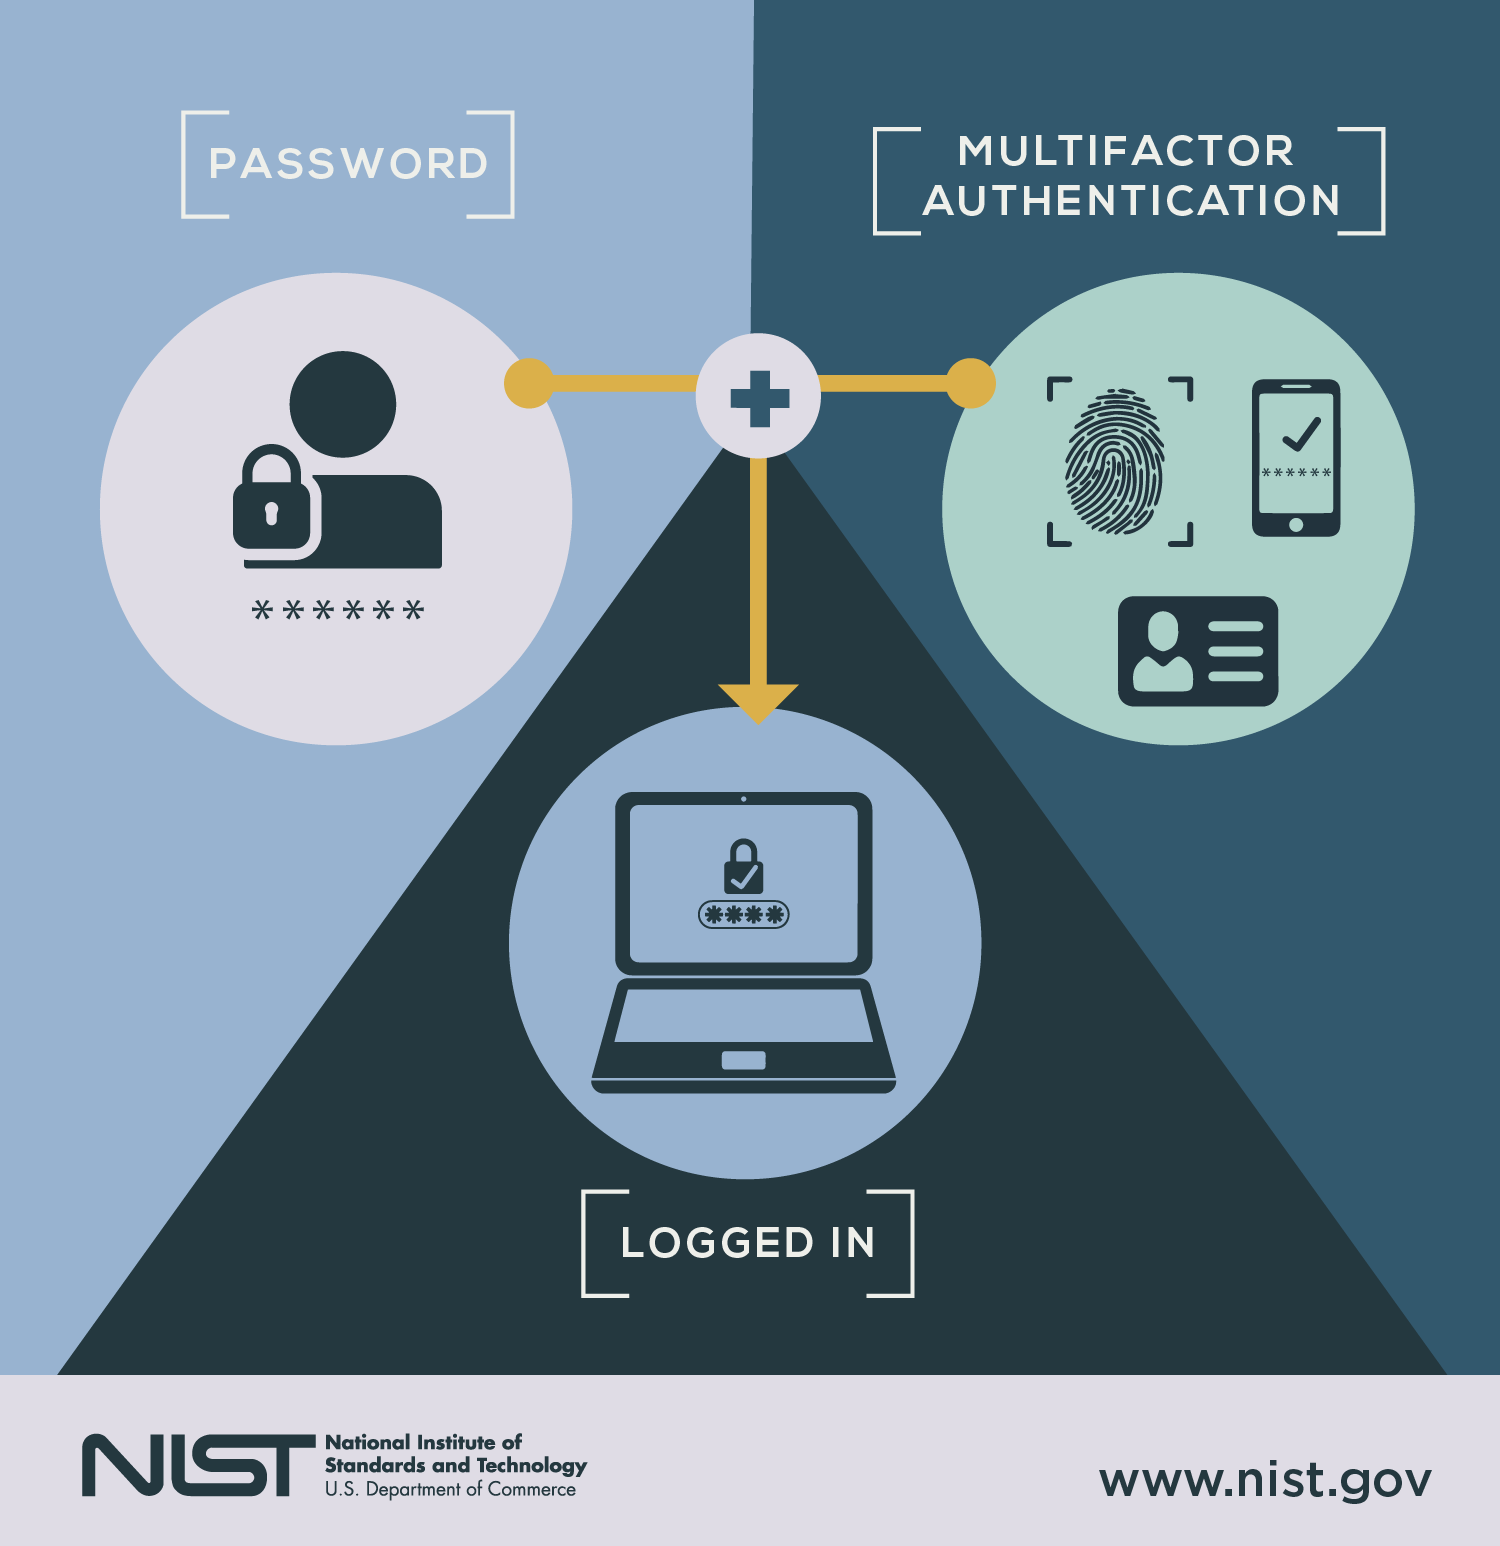
\includegraphics[width=15cm]{multifactor-authentificaton.png}

Ziel dieser Abschlussarbeit ist es, wie in dem Beispiel des \ac{nist} veranschaulicht, es eine Möglichkeit der sicheren und bequemen Authentifikation zu spezifizieren, die im Jahre 2020 keine utopischen Szenarien beschreibt, die die Voraussetzungen für eine sichere, bequeme und datenarme Authentifikation erfüllt. Ziel ist es auch, den Leser in die Sicht des Angreifers auf Systeme einzuweisen, sodass im Idealfall automatische Schutzreaktionen wie das Wählen von sicheren Passwörtern hervorgerufen, wenn nicht sogar eine der beschriebenen FIDO2 Verfahren wie der erste oder sogar der zweite Faktor, verwendet werden. Der Prototyp soll die verschiedenen Authentifizierungsmöglichkeiten veranschaulischen und präsentieren, um dem Nutzer die Wahl auf eines der Verfahren zu erleichtern. Gleichzeitig ist eines der Hauptziele dieser Arbeit auch die Grenzen von 'modernen' Authentifizierungsverfahren aufzuzeigen und auf dessen Nachteile hinzuweisen. Inwiefern eine Kombination dieser vorhandenen Verfahren, Probleme löst und welche minderen Probleme dabei entstehen soll ausführlich erläutert werden. Ein weiteres Ziel soll es sein, in gewisser weise kategorisch darzulegen, welches Verfahren für welchen Nutzertypen geeignet ist. Die Idee dahinter ist, dass es eine klare Trennung in der Nutzung von Accounts zwischen Entwicklern, Unternehmern und dem 'Casual Websurfer' gibt. Was alle drei Arten von Computernutzern allerdings gemeinsam haben ist: Sie besitzen persönliche Daten, an die kein Angreifer bzw. eben kein Dritter gelangen soll. Der Schutz dieser Daten sollte jedem Individuum selbst wichtig sein, um in den nächsten 5 bis 10 Jahren auf Besserung zu hoffen. Nicht nur technisch muss die Menscheit mit dem neuen digitalen Zeitalter umgehen und sich absichern können, sondern auch auf die menschliche Komponente muss von jedem selbst geachtet werden.

Es sollte dennoch erwähnt sein, dass diese Arbeit nicht darauf abzielt jede mögliche Authentifikationsstrategie zu durchläuchtern. Erläutern werden eher das klassiche User-ID und Passwort als Authentifikationsmöglichkeit und dem Gegenüber stehn die meistgenutzen Verfahren, die meist eher auf private Schlüssel oder die Kategorien 2 und 3 der Möglichkeiten zur Authentifizierung setzen. So ist der Yubikey am Ende nur eine Möglichkeit zur Umsetzung von einer Challenge-Response-basierten Authentikation anhand von privaten Schlüsseln welches bereits im FIDO Standart definiert ist. Auch ist es ein Nicht-Ziel dieser Arbeit das Resultat auf eine einzige perfekte Lösung zu dezimieren und diese zum neuen Standart zu erklären. Viel mehr soll es dem Leser durch eine tabellarische Auflistung von Vor- und Nachteilen jeder Methodik selbst überlassen sein, welche Methoden (und Tatempfehlungen dieser Arbeit) er für sich umsetzt.
